\documentclass[12pt]{article}
\usepackage{algorithm}
\usepackage{algpseudocode}
\usepackage{amsmath}
\usepackage{amssymb}
\usepackage{bm}
\usepackage{bbm}
\usepackage{color}
\usepackage{courier}
\usepackage{dsfont}
\usepackage{float}
\usepackage{geometry}
\usepackage{graphicx}
\usepackage{hyperref}
\usepackage{indentfirst}
\usepackage{listings,lstautogobble}
\usepackage{tikz}
\usetikzlibrary{decorations.markings}

\usepackage[mathscr]{euscript}
\hypersetup{
    colorlinks=true, %set true if you want colored links
    linktoc=all,     %set to all if you want both sections and subsections linked
    linkcolor=black,  %choose some color if you want links to stand out
}

% My matrix-related shorthands
% First three are easy (and nice-looking) ways to do different norms. In order: absolute value (one bar), vector norm (two bars), matrix norm (three bars). Ex: $\abs{x - y}$
% Next one is \ip for inner product. Ex: $\ip{x,y}$
% Last one is Trace used in the same way as the above.
\newcommand\abs[1]{\left|#1\right|}
\newcommand\norm[1]{\left\lVert#1\right\rVert}
\newcommand{\mnorm}[1]{{\left\vert\kern-0.25ex\left\vert\kern-0.25ex\left\vert #1 
    \right\vert\kern-0.25ex\right\vert\kern-0.25ex\right\vert}}
\newcommand\ip[1]{\left\langle#1\right\rangle}  
\newcommand{\tr}[1]{\text{tr}\left(#1\right)}
\newcommand{\vect}{\text{vec}}
\newcommand{\rank}{\text{rank}}
\renewcommand{\vec}[1]{\mathbf{#1}}

% Set
\newcommand\set[1]{\left\{#1\right\}}

% Convenient shorthands for your favorite \mathbb characters. \R for Reals, \C for Complex, \X for Abstract Spaces, \Ex for expected value, \Hil for Hilbert Spaces, and \ones for bold all-ones character.
\newcommand{\R}{\mathbb{R}}
\newcommand{\C}{\mathbb{C}}
\newcommand{\X}{\mathcal{X}}
\newcommand{\Ex}{\mathbb{E}}
\newcommand{\Hil}{\mathcal{H}}
\newcommand{\ones}{\mathbbm{1}}
\newcommand*{\vertbar}{\rule[-1ex]{0.5pt}{2.5ex}}
\newcommand*{\horzbar}{\rule[.5ex]{4ex}{0.5pt}}

% argmax and argmin defined similarly as \min and \max
\DeclareMathOperator*{\argmax}{arg\,max}
\DeclareMathOperator*{\argmin}{arg\,min}

% You can get those fancy bold font declarations by doing something like \begin{theorem}[<theorem title (optional)>] <body text> \end{theorem}
\newtheorem{theorem}{Theorem}[section]
\newtheorem{lemma}[theorem]{Lemma}
\newtheorem{proposition}[theorem]{Proposition}
\newtheorem{corollary}[theorem]{Corollary}
\newtheorem{observation}[theorem]{Observation}
\newtheorem{definition}[theorem]{Definition}
\newtheorem{remark}[theorem]{Remark}
\newtheorem{claim}[theorem]{Claim}

% Counter for align* environment
\newcommand\numberthis{\stepcounter{equation}\tag{\theequation}}

\geometry{margin=1in}
\setlength\parindent{30pt}

\title{VanillaCNN:\\Deriving Convolutional Neural Networks from Scratch}
\author{Ngan Vu \\ Final Project, S\&DS 430: Optimization Techniques, Yale University}

\begin{document}
\maketitle

\section{Introduction}
\subsection{What is a Convolutional Neural Network?}
\textbf{Convolutional Neural Network} (CNNs) are a class of \textbf{Deep Neural Networks} (DNNs) and are commonly used in image analysis tasks. Like all DNNs, CNNs aim to mimic the information processing and communication patterns in the \textbf{biological nervous system} - how neurons interact with one another to accomplish a task. CNNs, in particular, are inspired by the connectivity patterns of neurons specifically in the \textbf{animal visual cortex}, in which individual cortical neurons respond to stimuli only in a restricted region of the visual field known as the \textbf{receptive field}.

A CNN typically consists of an \textbf{input layer}, an \textbf{output layer}, and multiple \textbf{hidden layers}. The first hidden layers are typically pairs of \textbf{convolutional layers} and \textbf{pooling layers}. The last hidden layers are typically \textbf{fully connected layers}. On a high level:
\begin{itemize}
    \item \textbf{Convolutional layers} convolve one or more inputs (2D grids of cells) in the previous layer with one or more kernels, resulting in one or more outputs (2D grids of cells) in the next layer. The convolution operation is defined below.
    \item \textbf{Pooling layers} combine multiple cells from the input in the previous layer into one cell in the output in the next layer. The combination operation is typically summing, averaging, or taking the max.
    \item \textbf{Fully connected layers} connect every cell in the previous layer with every cell in the next layer. Each connection is assigned a weight, which specifies how much each input cell contributes to each output cell.
\end{itemize}

In each \textbf{learning iteration} (or \textbf{epoch}), an input is passed through the network in a process called \textbf{feed forward} to get a predicted output. The predicted output is then compared against the actual output to determine a \textbf{loss}. Then, the \textbf{gradient} of the loss is propagated back through the network in a process called \textbf{back propagation} to evaluate the \text{partial derivatives} of the parameters being learned (kernels, weights, and biases). Each parameter is then adjusted in the direction of negative partial derivative to reduce the loss. This method of following the negative gradient direction to minimize loss is called \textbf{gradient descent}. The whole process is repeated for many iterations until the loss converges, which suggests that a local minimum has been achieved.

\subsection{Motivation of this paper}
Currently, while there are a lot of materials on Convoluational Neural Networks available online, to my knowledge, none of them concretely derives how CNNs work and then implements a CNN using their derivation. Articles that go through the math of CNNs do not provide any implementation. This lack of accompanying code allows the notations to be somewhat lax, especially in indexing (for example, allowing negative indices in a matrix, or not starting the indices from the top-left corner of a matrix). Articles that actually implement their derivations only use toy data sets whose data points are very small ($2 \times 2$ or $3 \times 3$ images).

In practice, CNNs are usually built with Python packages and all operations (feed forward, loss evaluation, backpropagation, parameters update) are handled by these packages. Users of these packages do not necessarily understand how CNNs work behind the scene.

This paper aims to \textbf{concretely derives the math} behind Convolutional Neural Networks and then \textbf{implements an instance} of CNN using this derivation. With such a goal comes many stricter requirements, including but not limited to:
\begin{itemize}
    \item enforcing the consistency of the sizes of all inputs, outputs, kernels, weights, and biases
    \item starting all indices with 0 and allowing no negative indices
\end{itemize}
so that \textbf{all mathematical formulas can be translated directly to code}. I believe this step-by-step derivation, accompanied by executable code, is helpful for both beginners and experienced readers who want to understand CNN more thoroughly.

\section{Mathematical Background}
\subsection{Notations}
\noindent
- Vector: $\vec{v}$\\
- Matrix: $\bm{A}$\\
- Row $i$ of matrix: $\bm{A(i, :)}$; Column $j$ of matrix: $\bm{A(:, j)}$\\
- Convolution: $\bm{I} \ast \bm{K}$\\
- Correlation: $\bm{I} \star \bm{K}$\\
- Sigmoid function: $\sigma(x)$\\
- Pointwise product of matrices: $\bm{A} \odot \bm{B}$\\
- Dot product: $\bullet$\\
- Multiplication of scalars/matrices: $ab$ or $\bm{A}\bm{B}$, although sometimes $a \cdot b$ or $\bm{A}\cdot \bm{B}$ is used.\\
- Indexing: All indices start with 0 to follow the convention in most programming languages.\\
- Set of integers from $0$ to $N - 1$: $[N]$

\subsection{Correlation and Convolution}
In two dimensions, both \textbf{correlation} (also called cross-correlation) and \textbf{convolution} are processes of applying a 2D \textbf{kernel} on each cell of a 2D \textbf{input}, resulting in a 2D \textbf{output} that expresses how the input is modified by the kernel. The main difference between convolution and correlation is the \textbf{orientation of the kernel}.

We will discuss both operations below to see why it is actually better to replace the convolution operation in each convolutional layer of a CNN with the correlation operation, while not changing the functionality of the CNN.

\subsubsection{Definition}
With a $(x_i \times y_i)$ input $\bm{I}$, a $(x_k \times y_k)$ kernel $\bm{K}$, and a $(x_o \times y_o)$ output $\bm{O}$:
\begin{itemize}
    \item The formula for the \textbf{correlation} is:
    \begin{align*}
        \bm{O}(i, j) = \bm{I} \star \bm{K} = \sum_{u = 0}^{x_k - 1}\sum_{v = 0}^{y_k - 1} \bm{I}(i + u, j + v)\bm{K}(u, v) \quad \forall i \in [x_o], j \in [y_o]
        \numberthis \label{correlation}
    \end{align*}
    \item The formula for the \textbf{convolution} is:
    \begin{align*}
        \bm{O}(i, j) = \bm{I} \ast \bm{K} = \sum_{u = 0}^{x_k - 1}\sum_{v = 0}^{y_k - 1} \bm{I}(i - u, j - v)\bm{K}(u, v) \quad \forall i \in [x_o], j \in [y_o]
        \numberthis \label{convolution}
    \end{align*}  
\end{itemize}
Correlation of $\bm{I}$ and $\bm{K}$ is actually equivalent to convolution of $\bm{I}$ and $\bm{K_{rot}}$, where $\bm{K_{rot}}$ is $\bm{K}$ rotated by $180^o$. This is because:
\begin{align*}
    \bm{K}_{rot}(u, v) &= \bm{K}(x_k - 1 - u, y_k - 1 - v)\\
    \bm{O}_{conv}(i, j) &= \sum_{u = 0}^{x_k - 1}\sum_{v = 0}^{y_k - 1} \bm{I}(i - u, j - v)\bm{K}(u, v)\\
    &= \sum_{(x_k - 1 - u) = 0}^{x_k - 1}\sum_{(y_k - 1 - v) = 0}^{y_k - 1} \bm{I}(i - (x_k - 1 - u), j - (y_k - 1 - v))\bm{K}(x_k - 1 - u, y_k - 1 - v)\\
    &\quad\,\, (\text{replace } u \text{ with } (x_k - 1 - u) \text{ and } v \text{ with } (y_k - 1 - v))\\
    &= \sum_{u = 0}^{x_k - 1}\sum_{v = 0}^{y_k - 1} \bm{I}((i - x_k - 1)+ u , (j - y_k - 1) + v)\bm{K}_{rot}(u, v)\\
    &\quad\,\, \text{(rewrite the bounds with the exactly equivalent bounds)}\\
    &= \bm{O}_{corr}((i - x_k - 1), (j - y_k - 1))
\end{align*}
As we could see, there is a bijective mapping between $\bm{O}_{conv}$ and $\bm{O}_{corr}$. The difference in indices is due to the complication in indexing in convolution using the formula above; this complication is addressed below. The final results of $\bm{I} \ast \bm{K}$ and $\bm{I} \star \bm{K_{rot}}$ should be exactly the same.

\subsubsection{Why replace convolution with correlation?}
The main purpose of this section is to explain why I use correlation instead of convolution in my derivation and implementation of CNNs. We saw above that convolution is just correlation with the kernel rotated {$180^o$}. This section shows that correlation is easier to implement than convolution and therefore if we can replace convolution with correlation, we should do so.

Let's look at the indices and the shapes of the input $\bm{I}$, output $\bm{O}$, and kernel $\bm{K}$.
\begin{itemize}
    \item Correlation:\\
    According to equation \eqref{correlation}, to make sure that the indices of $\bm{I}$ is not out of bound and that all indices in $\bm{I}$ is touched, we require that:
    \begin{itemize}
        \item $\forall i \in [x_o], u \in [x_k]: 0 \leq i + u \leq x_i - 1$\\
        \quad $\Rightarrow
        \begin{cases}
        0 = \min{(i)} + \min{(u)} = 0 + 0, \text{ already satisfied}\\
        x_i - 1 = \max{(i)} + \max{(u)} = (x_o - 1) + (x_k - 1) = x_o + x_k - 2
        \end{cases}
        $\\
        \quad $\Rightarrow x_o = x_i - x_k + 1$
        \item $\forall j \in [y_o], v \in [y_k]: 0 \leq j + v \leq y_j - 1$\\
        \quad $\Rightarrow
        \begin{cases}
        0 = \min{(i)} + \min{(u)} = 0 + 0, \text{ already satisfied}\\
        y_i - 1 = \max{(j)} + \max{(v)} = (y_o - 1) + (y_k - 1) = y_o + y_k - 2
        \end{cases}
        $\\
        \quad $\Rightarrow y_o = y_i - y_k + 1$
    \end{itemize}
    \item Convolution:\\
    Note that because there is subtraction, for the convolution formula to work in our implementation, we need to make either of these two sacrifices in indexing:
    \begin{itemize}
        \item Indices of $\bm{I}$ are non-negative, but indices of $\bm{O}$ do not start at 0 (they start at $x_k - 1$ and $y_k - 1$). In this case:
        \begin{itemize}
            \item For $\bm{I}$: 
            $\begin{cases}
            0 \leq i - u \leq x_i - 1\\
            0 \leq j - v \leq y_i - 1
            \end{cases}$
            (normal indices)
            
            \item For $\bm{O}$:
            $\begin{cases}
            x_k - 1 \leq i \leq x_o + x_k - 2\\
            y_k - 1\leq j \leq y_o + y_k - 2
            \end{cases}$
            (shift indices up by $(x_k - 1, y_k - 1)$)
        \end{itemize}
        \item Indices of $\bm{O}$ do start at 0, but indices of $\bm{I}$ are not non-negative (they start at $- x_k + 1$ and $-y_k + 1$). In this case:
        \begin{itemize}
            \item For $\bm{I}$: 
            $\begin{cases}
            -x_k + 1 \leq i - u \leq x_i - x_k\\
            -y_k + 1\leq j - v \leq y_i - y_k
            \end{cases}$
            (shift indices down by $(x_k - 1, y_k - 1)$)
            
            \item For $\bm{O}$:
            $\begin{cases}
            0 \leq i \leq x_o - 1\\
            0 \leq j \leq y_o - 1
            \end{cases}$
            (normal indices)
        \end{itemize}
    \end{itemize}
    
    We will use the second option so that we have $i \in [x_o], j \in [y_o] $.\\
    According to equation \eqref{convolution}, to make sure that the indices of $\bm{I}$ is not out of bound and that all indices in $\bm{I}$ is touched, we require that:
    \begin{itemize}
        \item $\forall i \in [x_o], u \in [x_k]: -x_k + 1\leq i + u \leq x_i - x_k$\\
        \quad $\Rightarrow
        \begin{cases}
        -x_k + 1 = \min{(i)} - \max{(u)} = 0 - (x_k + 1), \text{ already satisfied}\\
        x_i - x_k = \max{(i)} - \min{(u)} = (x_o - 1) - 0 = x_o - 1
        \end{cases}
        $\\
        \quad $\Rightarrow x_o = x_i - x_k + 1$
        \item $\forall j \in [y_o], v \in [y_k]: -y_k + 1 \leq j + v \leq y_i - y_k$\\
        \quad $\Rightarrow
        \begin{cases}
        -y_k + 1 = \min{(i)} + \min{(u)} = 0 - (y_k - 1), \text{ already satisfied}\\
        y_i - y_k = \max{(j)} + \min{(v)} = (y_o - 1) - 0 = y_o - 1
        \end{cases}
        $\\
        \quad $\Rightarrow y_o = y_i - y_k + 1$
    \end{itemize}
\end{itemize}

In both operations, the shape of $\bm{O}$ given $\bm{I}$ and $\bm{K}$ is $(x_o, y_o) = (x_i - x_k + 1, y_i - y_k + 1)$. However, it is evident that indexing in correlation is a lot cleaner than indexing in convolution. Correlation also follows how indexing works in most programming languages (indices of an array of size $N$ should go from $0$ to $N - 1$). To meet the strict requirements of array indexing in coding, I replace convolution with correlation in the derivation below and in the implementation of a CNN. The kernels learned by the CNN using this implementation can be thought of as the $180^o$-rotated versions of kernels that the CNN would have learned had I not changed convolution to correlation.

\subsubsection{Padding}
In the formulas above, for both correlation and convolution, the shape of the output is smaller than that of the input ($(x_o, y_o) = (x_i - x_k + 1, y_i - y_k + 1)$). If we think of correlation and convolution as sliding a kernel on top of the input, with these formulas, we need to ensure that the kernel never goes beyond the edges of the input. As a result, for any kernel of size larger than $(1 \times 1)$, the range of indices that can be the top-left of a kernel is smaller than the range of indices of the input matrix, as they have to account for width and height of the kernel. Therefore, the output matrix is smaller than the matrix.

In certain cases, it can be useful to pad the input matrix with all-zero edges, resulting in an output of a shape larger than that of the input. We will see later that \textbf{during feed forward, correlation without padding should be used}, while \textbf{during back propagation, convolution with padding should be used}. This makes sense in terms of:
\begin{itemize}
    \item \textbf{Shapes}: if during feed forward, we reduce the shape of input $\bm{I}$ to the shape of output $\bm{O}$ by not using padding, then during back propagation (which moves in the exact opposite direction) we need to enlarge $\bm{O}$ to the shape of $\bm{I}$ by using padding.
    \item \textbf{Indexing}: See the figure below. In feed forward $\bm{I}(0, 0)$ only contributes to $\bm{O}(0, 0)$ and no other output cells. In back propagation, $\bm{I}(0, 0)$ only receives contribution from $\bm{O}(0, 0)$ and no other output cells. This is true for all other input cells on the edges: they only receive the propagation of loss gradient from output cells they contribute to.
\end{itemize}
\begin{center}
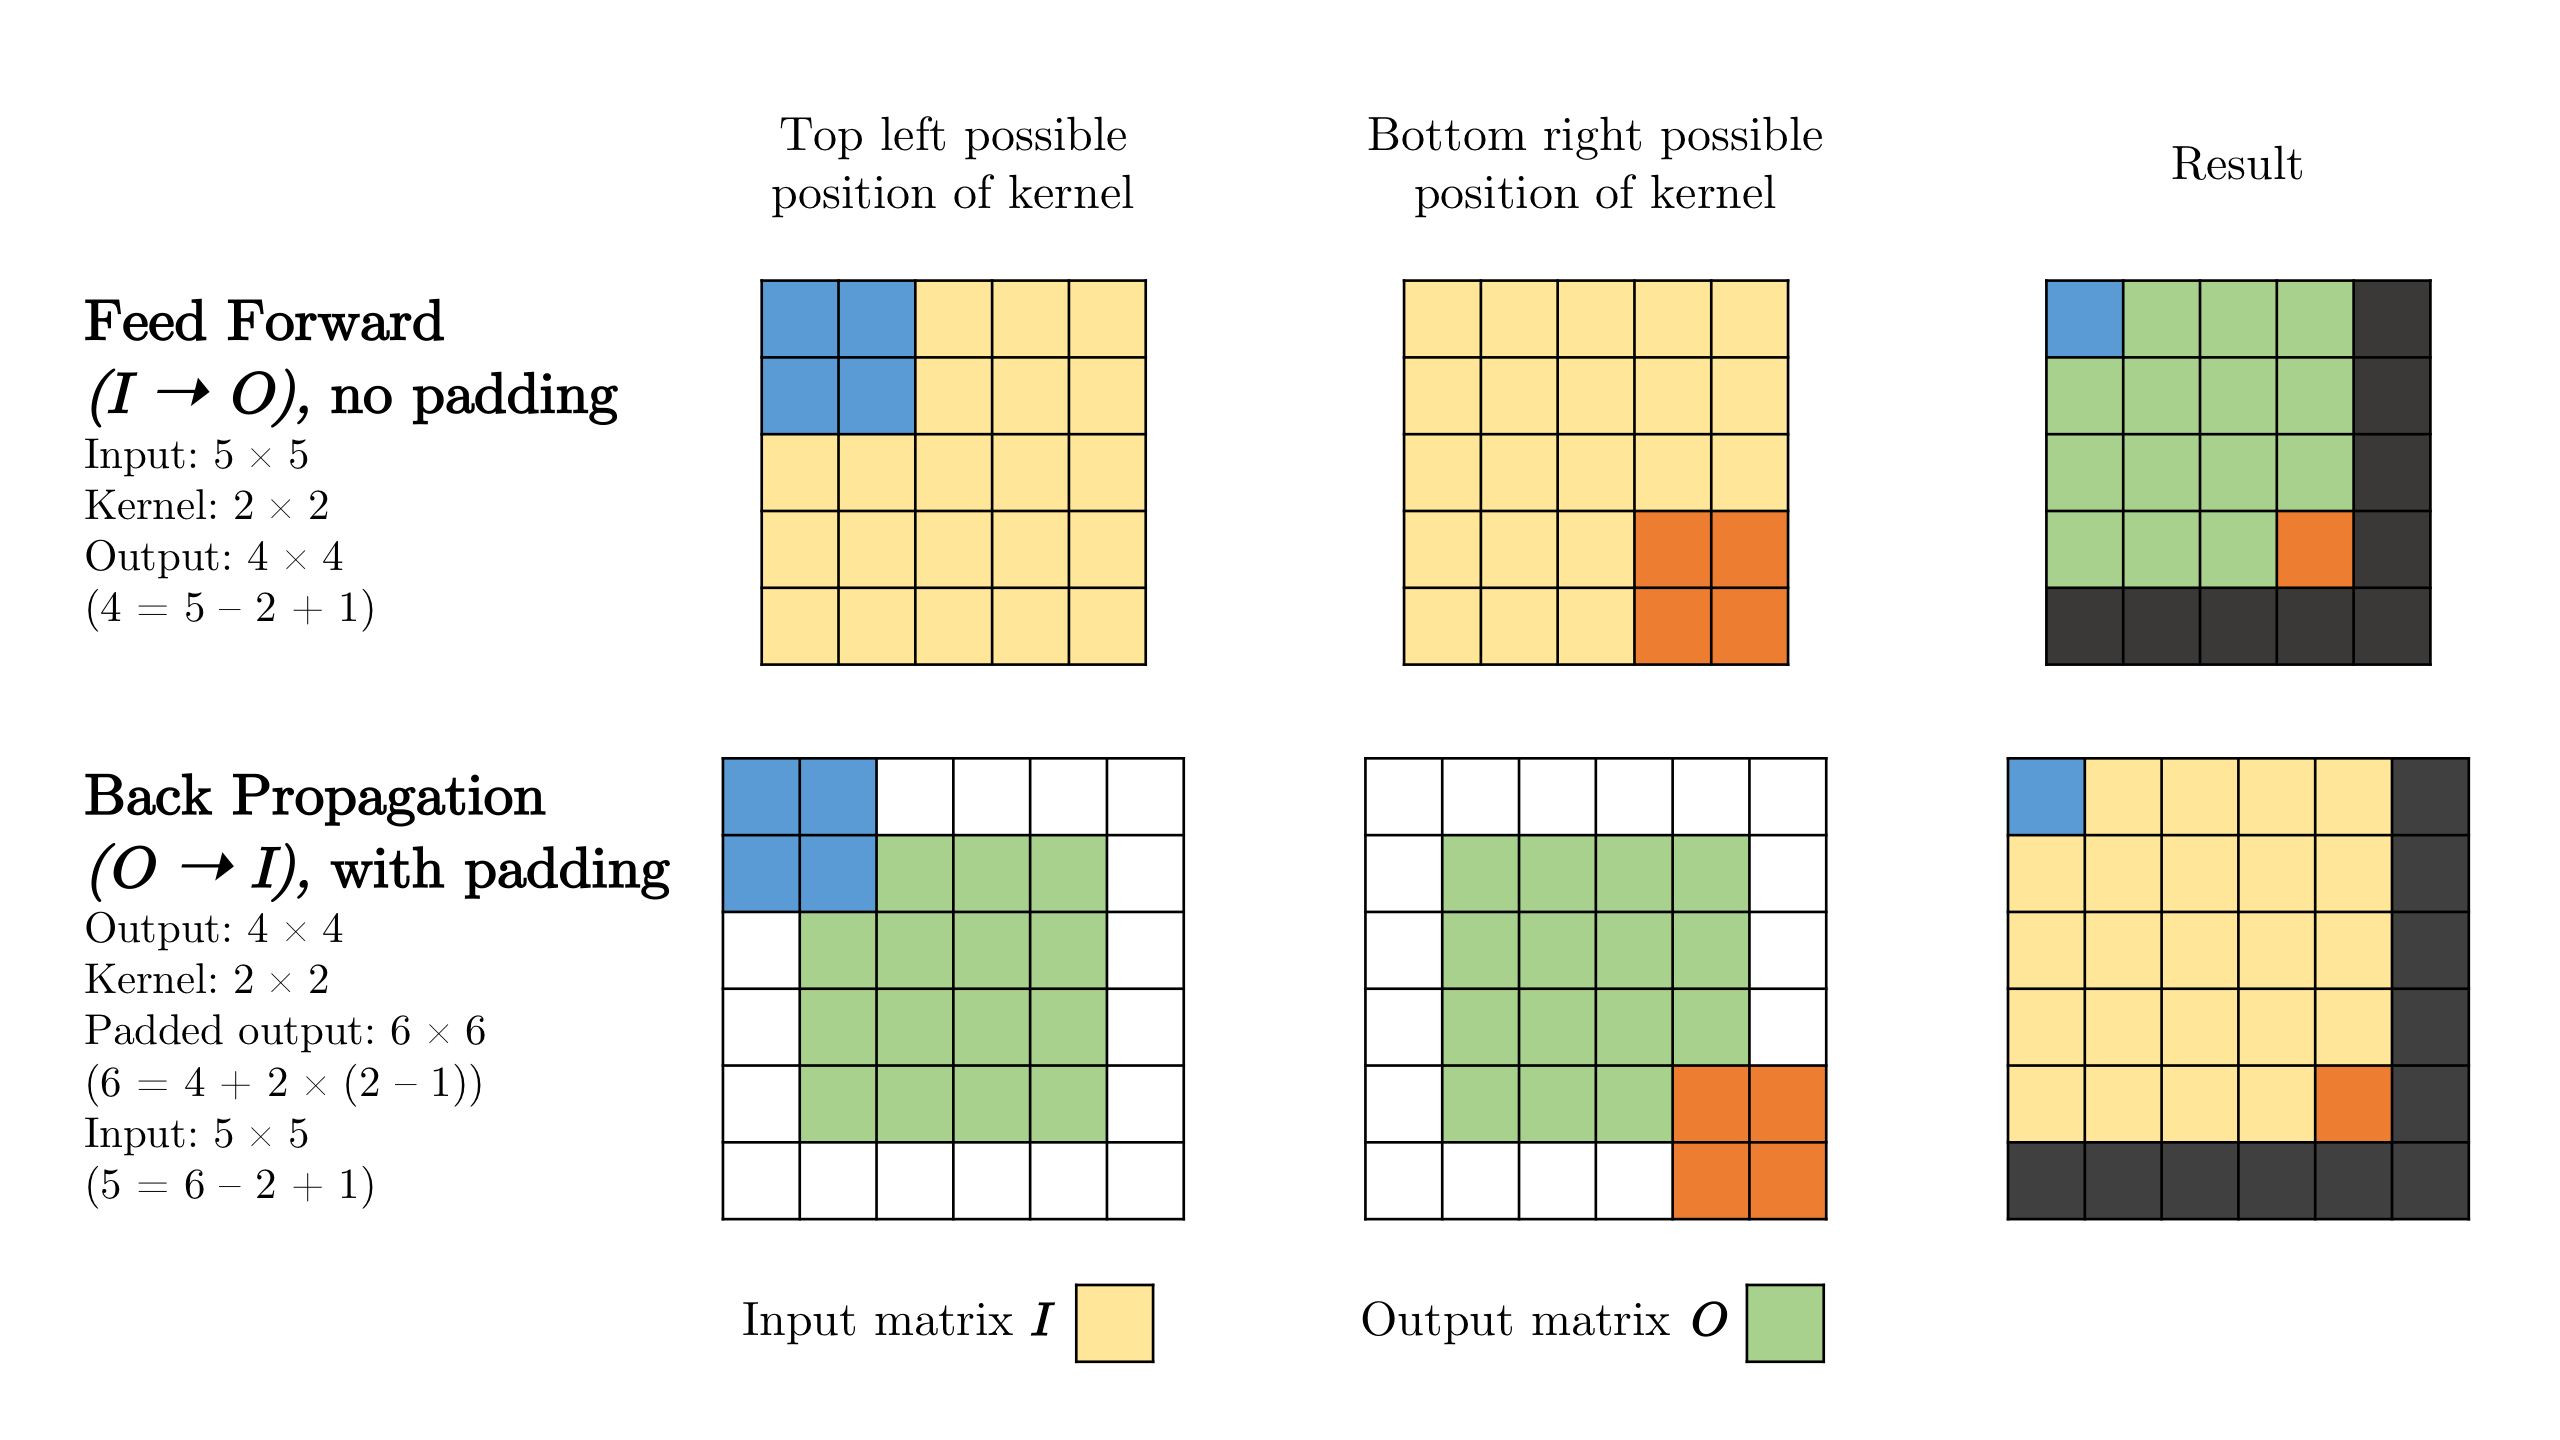
\includegraphics[width=\textwidth]{padding.png}
\textit{Feed Forward with no padding and Back Propagation with padding\\ preserve consistency in the shapes of input and output matrices}
\end{center}

When padding is used:
\begin{itemize}
\item The shape of the padded input is:
$$(x_{pad, i}, y_{pad, i}) = (x_i + 2(x_k - 1), y_i + 2(y_k - 1))$$
This is because we add $(x_k - 1)$ rows to each of the top and bottom edges, and $(y_k - 1)$ to each of the left and right edges, just enough so that the kernel matrix can have at least one overlapping cell with the non-padded input matrix.
\item The modified formula for convolution is:
\begin{align*}
\bm{O}(i, j) &= \sum_{u = 0}^{x_k}\sum_{v = 0}^{y_k} \bm{I}_{pad}(i - u, j - v)\bm{K}(u, v) \quad \forall i \in [x_o], j \in [y_o]
\\
\text{where }
\bm{I}_{pad}(i - u, j - v) &= 
\begin{cases}
    \bm{I}(i - u, j - v) \text{ if } 0 \leq i - u \leq x_i, 0 \leq j - v \leq y_i\\
    0 \text{ otherwise}
\end{cases}
\numberthis \label{convolution_padding}
\end{align*}
By adding padding,  we can allow $(i - u, j - v)$ to be out of $\bm{I}$'s bounds: all out-of-bound indices are defined to be 0. Padding extends $\bm{I}$'s bounds from:
\begin{align*}
    0 \leq i - u \leq x_i - 1\\
    0 \leq j - v \leq y_i - 1
\end{align*}
to $\bm{I_{pad}}$'s bounds:
\begin{align*}
    -(x_k - 1) \leq i - u \leq x_i - 1 + (x_k - 1)\\
    -(y_k - 1) \leq j - v \leq y_i - 1 + (y_k - 1)
\end{align*}
\end{itemize}

According to equation \eqref{convolution_padding}, to make sure that the indices of $\bm{I}$ is not out of bound and that all indices in $\bm{I}$ is touched, we require that:
\begin{itemize}
    \item $\forall i \in [x_o], u \in [x_k]: -(x_k - 1)\leq i + u \leq x_i - 1 + (x_k - 1)$\\
    \quad $\Rightarrow
    \begin{cases}
    -(x_k - 1) = \min{(i)} - \max{(u)} = 0 - (x_k - 1), \text{ already satisfied}\\
    x_i - 1 + (x_k - 1) = \max{(i)} - \min{(u)} = (x_o - 1) - 0 = x_o - 1
    \end{cases}
    $\\
    \quad $\Rightarrow x_o = x_i + x_k - 1$
    \item $\forall j \in [y_o], v \in [y_k]: -y_k + 1 \leq j + v \leq y_i - y_k$\\
    \quad $\Rightarrow
    \begin{cases}
    -(y_k - 1) = \min{(j)} - \max{(v)} = 0 - (y_k + 1), \text{ already satisfied}\\
    y_i -  1 + (y_k - 1) = \max{(j)} - \min{(v)} = (y_o - 1) - 0 = y_o - 1
    \end{cases}
    $\\
    \quad $\Rightarrow y_o = y_i + y_k - 1$
\end{itemize}
To recap, the shape of output matrix when padding is not used is:
\begin{align*}
    (x_o, y_o) =  (x_i - x_k + 1, y_i - y_k + 1)
    \numberthis \label{no_padding_shape}
\end{align*}
while the shape of output matrix when padding is used is:
\begin{align*}
    (x_o, y_o) = (x_i + x_k - 1, y_i + y_k - 1)
    \numberthis \label{padding_shape}
\end{align*}
\subsection{Sigmoid function}
Sigmoid function is a function with the characteristic S-shaped curve. It is widely used in neural network as an activation function, which models whether a neuron should fire (output a 1) or not fire (output a 0), given any input. It is usually applied right after the convolutional layer and right after the fully connected layer.
\begin{center}
    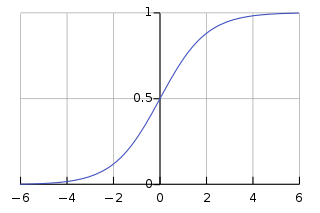
\includegraphics[width=150px]{sigmoid.png}\\
    \textit{Sigmoid function}
\end{center}
The function is defined as:
\begin{align*}
    \sigma(x) = \frac{e^x}{e^x + 1} = \frac{1}{1 + e^{-x}}
\end{align*}
Let's consider the derivative of this function. Define:
\begin{align*}
    f(x) = \frac{1}{\sigma{(x)}} = 1 + e^{-x}
\end{align*}
On one hand:
\begin{align*}
    f'(x) = \frac{\partial}{\partial x}\left( \frac{1}{\sigma{(x)}}\right) = -\frac{\sigma'{(x)}}{\sigma^2{(x)}}
\end{align*}
On the other hand:
\begin{align*}
    f'(x) = \frac{\partial}{\partial x}\left( 1 + e^{-x}\right) = -e^{-x} = 1 - f(x) = 1 - \frac{1}{\sigma{(x)}} = \frac{\sigma{(x)} - 1}{\sigma{(x)}}
\end{align*}
Equating the two equations, we have:
$
-\frac{\sigma'{(x)}}{\sigma^2{(x)}} &= \frac{\sigma{(x)} - 1}{\sigma{(x)}}
$
\begin{align*}
\Leftrightarrow \sigma'{(x)} &= (\sigma{(x)})(1 - \sigma{(x)})
\numberthis \label{sigmoid_derivative}
\end{align*}
We will use this formula for the derivative of the sigmoid function in the derivation below.

\section{Architecture of Convolutional Neural Networks}
\begin{center}
    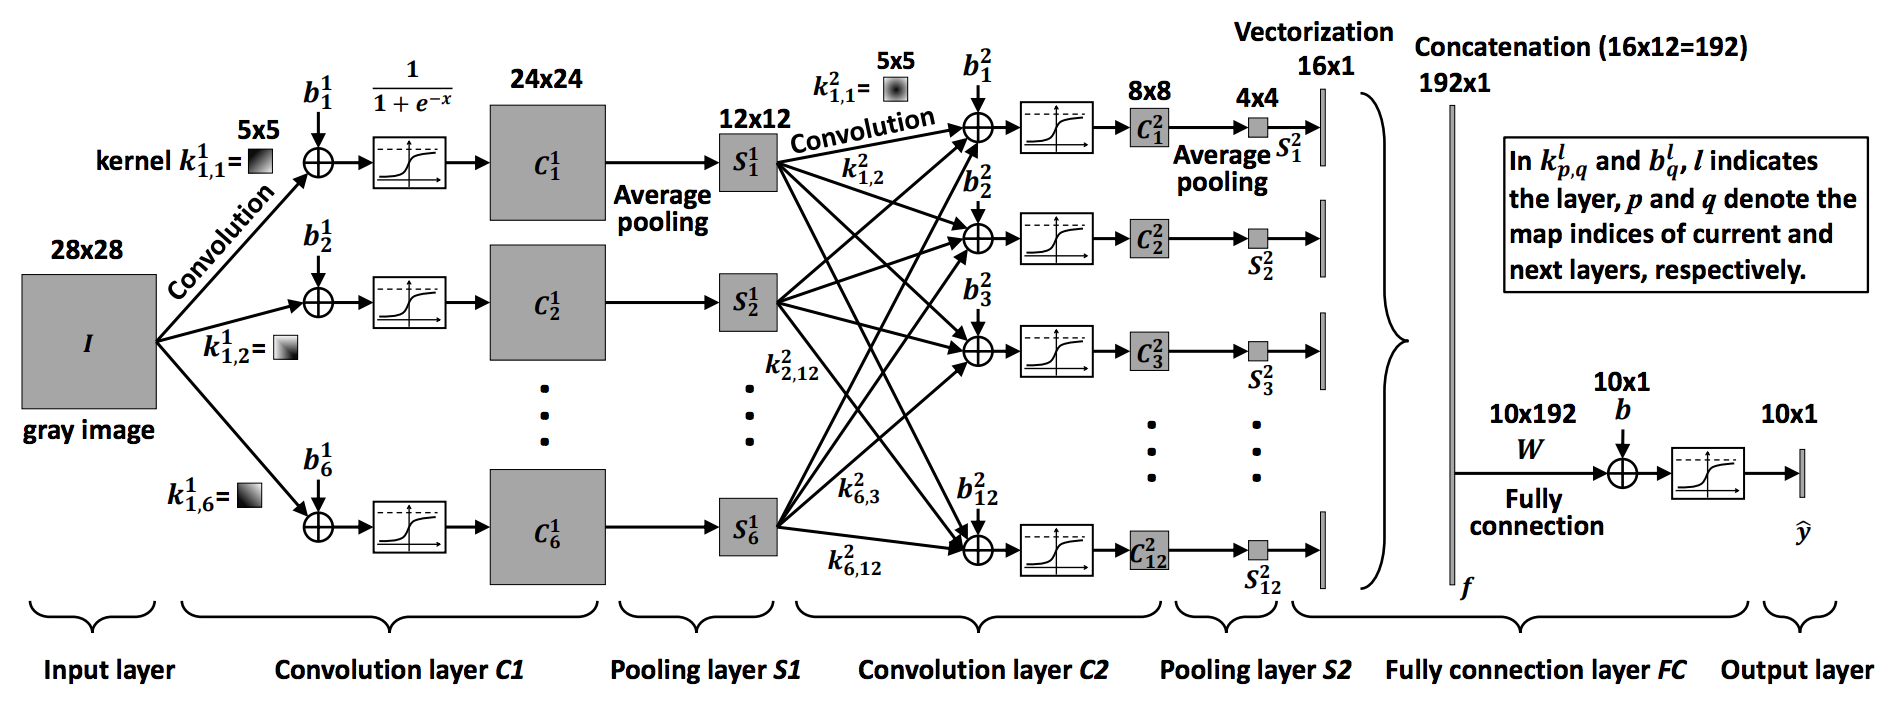
\includegraphics[width=\textwidth]{CNN-architecture.png}\\
    \textit{Architecture of the CNN used in this paper}
\end{center}
The Convolutional Neural Network that we will use in this paper is described in the figure above. It has the same structure as the demo of Matlab DeepLearnToolbox. It takes in \textbf{28 $\times$ 28 inputs} and returns \textbf{10 $\times$ 1 outputs}. Thus, this CNN can be used to \textbf{classify handwritten digits} in the \textbf{MNIST} data set, which consists of \textbf{28 $\times$ 28 images} of digits belonging to \textbf{10 classes} (digits $0$ to $9$).
\begin{center}
    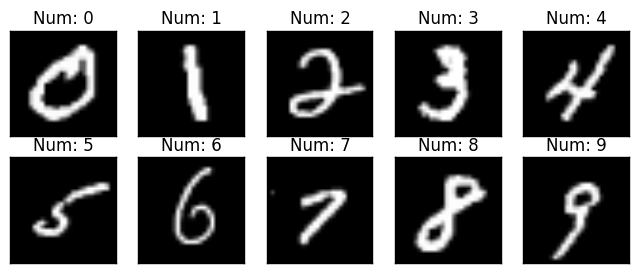
\includegraphics[width=280px]{mnist.png}\\
    \textit{MNIST data set}
\end{center}

\section{Deriving Feed Forward and Back Propagation}
\subsection{Parameters Initialization}
\subsubsection{Convolutional Layer 1}
$\forall p \in [6]$, $\bm{K}^1_{1,p}$ is a $(5 \times 5)$ matrix and $b^1_p$ is a $(1 \times 1)$ scalar, initialized as:
\begin{align*}
    \bm{K}^1_{1,p} &\sim U\left(\pm \sqrt{\frac{6}{(1 + 6) \times 5^2}}\right)
    \numberthis
    \\
    b^1_p &= 0
    \numberthis
\end{align*}
\subsubsection{Convolutional Layer 2}
$\forall p \in [6], q \in [12]$, $\bm{K}^2_{p,q}$ is a $(5 \times 5)$ matrix and $b^2_q$ is a $(1 \times 1)$ scalar, initialized as:
\begin{align*}
    \bm{K}^2_{p,q} &\sim U\left(\pm \sqrt{\frac{6}{(6 + 12) \times 5^2}}\right)
    \numberthis
    \\
    b^2_q &= 0
    \numberthis
\end{align*}
\subsubsection{Fully Connected Layer}
$\bm{W}$ is a $(10 \times 192)$ matrix and $\vec{b}$ is a $(10 \times 1)$ scalar, initialized as:
\begin{align*}
    \bm{W} &\sim U\left(\pm \sqrt{\frac{6}{192 + 10}}\right)
    \numberthis
    \\
    \vec{b} &= \vec{0}
    \numberthis
\end{align*}

\subsection{Feed Forward}
\subsubsection{Convolutional Layer 1: $\textbf{\textit{I}} \rightarrow \textbf{\textit{C}}^1_\sigma$}

\begin{align*}
    \bm{I}:& \text{ input}, 28 \times 28 \text{ matrix}\\
    \bm{K}^1_{1, p}, p \in [6]:& \text{ kernel}, 5 \times 5 \text{ matrix}\\
    \bm{B}^1_p, p \in [6]:& \text{ bias}, 24 \times 24 \text{ matrix whose all entries are of the same value}, b^1_p\\
    \bm{C}^1_p, p \in [6]:& \text{ output before non-linearity}, 24 \times 24 \text{ matrix}\\
    \bm{C}^1_{\sigma, p}, p \in [6]:& \text{ output after non-linearity}, 24 \times 24 \text{ matrix}
\end{align*}

$\forall p \in [6]$, we have:
\begin{align*}
    \bm{C}^1_p &= \bm{I} \star \bm{K}^1_{1, p} + \bm{B}^1_p
    \numberthis \label{C1}
    \\
    \Leftrightarrow \bm{C}^1_p(i, j) &= \sum_{u = 0}^3\sum_{v = 0}^3\Big(\bm{I}(i + u, j + v)\bm{K}^1_{1,p}(u, v)\Big) + b^1_p \quad \forall i, j \in [24]
    \numberthis \label{C1_indexbased}
    \\
    &\quad(\text{based on correlation equation } \eqref{correlation})
    \\
    \bm{C}^1_{\sigma, p} &= \sigma(\bm{C}^1_p)
    \numberthis \label{C1_sigma}
\end{align*}

\subsubsection{Pooling Layer 1: $\textbf{\textit{C}}^1_\sigma \rightarrow \textbf{\textit{S}}^1$}

\begin{align*}
    \bm{C}^1_{\sigma, p}, p \in [6]:& \text{ input}, 24 \times 24 \text{ matrix}\\
    \bm{S}^1_p, p \in [6]:& \text{ output}, 12 \times 12 \text{ matrix}
\end{align*}

$\forall p \in [6]$, we have:
\begin{align*}
    \bm{S}^1_p(i, j) = \frac{1}{4}\sum_{u = 0}^1\sum_{v = 0}^1\bm{C}^1_{\sigma, p}(2i + u, 2j + v) \quad \forall i, j \in [12]
    \numberthis \label{S1}
\end{align*}

\subsubsection{Convolutional Layer 2: $\textbf{\textit{S}}^1 \rightarrow \textbf{\textit{C}}^2_\sigma$}

\begin{align*}
    \bm{S}^1_p, p \in [6]:& \text{ input}, 12 \times 12 \text{ matrix}\\
    \bm{K}^2_{p, q}, p \in [6], q \in [12]:& \text{ kernel}, 5 \times 5 \text{ matrix}\\
    \bm{B}^2_q, q \in [12]:& \text{ bias}, 8 \times 8 \text{ matrix whose all entries are of the same value}, b^2_q\\
    \bm{C}^2_q, q \in [12]:& \text{ output before non-linearity}, 8 \times 8 \text{ matrix}\\
    \bm{C}^2_{\sigma, q}, q \in [12]:& \text{ output after non-linearity}, 8 \times 8 \text{ matrix}
\end{align*}

$\forall q \in [12]$, we have:
\begin{align*}
    \bm{C}^2_q &= \sum_{p = 0}^5\Big(\bm{S}^1_p \star  \bm{K}^2_{p, q}\Big) + \bm{B}^2_q
    \numberthis \label{C2}
    \\
    \Leftrightarrow \bm{C}^2_q(i, j) &= \sum_{p = 0}^5\left(\sum_{u = 0}^3\sum_{v = 0}^3\bm{S}^1_p(i + u, j + v)\bm{K}^2_{p, q}(u, v)\right) + b^2_q \quad \forall i, j \in [8]
    \numberthis \label{C2_indexbased}
    \\
    &\quad(\text{based on correlation equation } \eqref{correlation})
    \\
    \bm{C}^2_{\sigma, q} &= \sigma(\bm{C}^2_q)
    \numberthis \label{C2_sigma}
\end{align*}

\subsubsection{Pooling Layer 2: $\textbf{\textit{C}}^2_\sigma \rightarrow \textbf{\textit{S}}^2$}
\begin{align*}
    \bm{C}^2_{\sigma, q}, q \in [12]:& \text{ input}, 8 \times 8 \text{ matrix}\\
    \bm{S}^2_q, q \in [12]:& \text{ output}, 4 \times 4 \text{ matrix}
\end{align*}
$\forall q \in [12]$, we have:
\begin{align*}
    \bm{S}^2_q(i, j) = \frac{1}{4}\sum_{u = 0}^1\sum_{v = 0}^1\bm{C}^2_{\sigma, q}(2i + u, 2j + v) \quad \forall i, j \in [4]
    \numberthis \label{S2}
\end{align*}

\subsubsection{Vectorization and Concatenation: $\textbf{\textit{S}}^2 \rightarrow \vec{v}$}
\begin{align*}
    \bm{S}^2_q, q \in [12]:& \text{ input}, 4 \times 4 \text{ matrix}\\
    \vec{v}:& \text{ output}, 192 \times 1 \text{ vector}
\end{align*}
$S^2_q$ is an array of kernels. To visualize $S^2_q$, let's pretend that it has only 2 kernels, each of which is of size $2 \times 2$:
\begin{align*}
    \begin{pmatrix}
        \begin{pmatrix}
        1 & 2\\
        3 & 4
        \end{pmatrix}\\
        \begin{pmatrix}
        5 & 6\\
        7 & 8
        \end{pmatrix}
    \end{pmatrix}
\end{align*}
After vectorizing $S^2_q$, we want to get:
\begin{align*}
    \begin{pmatrix}
        1 \\ 2 \\ 3 \\ 4 \\ 5 \\ 6 \\ 7 \\ 8
    \end{pmatrix}
\end{align*}
This is equivalent to "unrolling" each kernel in $S^2_q$ into a vector by going row by row, then combined the unrolled kernel into a long vector.\\
Now, let's define the concrete formula for this operation. We first vectorize each matrix $S^2_q$.\\
$\forall q \in [12]$, we have:
\begin{align*}
    \vec{v}_q &= \begin{pmatrix} | \\ \bm{S}^2_q(0, :)\top \\ | \\ ... \\ | \\ \bm{S}^2_q(3, :)^\top \\ | \end{pmatrix}\\
    \Leftrightarrow \vec{v}_q(4i + j) &= \bm{S}^2_q(i, j) \quad \forall i, j \in [4]
    \numberthis \label{vectorization}
\end{align*}
Now, we will concatenate the vectorized matrices into one long matrix.
\begin{align*}
    \vec{v} &= \begin{pmatrix} | \\ \vec{v}_1 \\ | \\ ... \\ | \\ \vec{v}_{12} \\ | \end{pmatrix}\\
    \Leftrightarrow \vec{v}(16q + 4i + j) &= \bm{S}^2_q(i, j) \quad \forall q \in [12], \forall i, j \in [4]
    \numberthis \label{concatenation}
\end{align*}

\subsubsection{Fully Connected Layer: $\vec{v} \rightarrow \vec{\hat{y}}_\sigma$}
\begin{align*}
    \vec{v}:& \text{ input}, 192 \times 1 \text{ vector}\\
    \bm{W}:& \text{ weights}, 10 \times 192 \text{ matrix}\\
    \vec{b}:& \text{ bias}, 10 \times 1 \text{ vector of independent values (unlike the biases above)}\\
    \vec{\hat{y}}:& \text{ output before non-linearity}, 10 \times 1 \text{ vector}\\
    \vec{\hat{y}_\sigma}:& \text{ output after non-linearity}, 10 \times 1 \text{ vector}
\end{align*}
\begin{align*}
    \vec{\hat{y}} &= \bm{W}\vec{v} + \vec{b}
    \numberthis \label{y_hat}
    \\
    \Leftrightarrow
    \vec{\hat{y}}(i) &= \sum_{j = 0}^{191}\Big(\bm{W}(i, j)\vec{v}(j)\Big) + \vec{b}(i)
    \numberthis \label{y_hat_indexbased}
    \\
    \vec{\hat{y}}_\sigma &= \sigma(\hat{y})
    \numberthis \label{y_hat_sigma}
\end{align*}

\subsection{Loss Evaluation}
\begin{align*}
    \vec{\hat{y}_\sigma}:& \text{ predicted labels}, 10 \times 1 \text{ vector}\\
    \vec{y}:& \text{ actual labels}, 10 \times 1 \text{ vector}\\
    L:& \text{ loss}, 1 \times 1 \text{ scalar}
\end{align*}
\begin{align*}
    L = \frac{1}{2} \norm{\vec{\hat{y}}_\sigma - \vec{y}}^2 =  \frac{1}{2}\sum_{i=0}^{9}(\vec{\hat{y}}_\sigma(i) - \vec{y}(i))^2
    \numberthis \label{loss}
\end{align*}

\subsection{Back Propagation}
\subsubsection{Fully Connected Layer: $\vec{\hat{y}}_\sigma \rightarrow \vec{v}$}
\begin{itemize}

\item Calculating $\Delta{\vec{\hat{y}}_\sigma}$
\begin{align*}
    \Delta{\vec{\hat{y}}_\sigma}:& \text{ partial w.r.t predicted labels after non-linearity}, 10 \times 1 \text{ vector}\\
    {\vec{\hat{y}}_\sigma}:& \text{ predicted labels after non-linearity}, 10 \times 1 \text{ vector}\\
    {\vec{y}}:& \text{ actual labels}, 10 \times 1 \text{ vector}
\end{align*}
\begin{align*}
    \Delta{\vec{\hat{y}}_\sigma}(i)
    &= \frac{\partial{L}}{\partial{\vec{\hat{y}}_\sigma}(i)}
    \\
    &= \frac{\partial}{\partial{\vec{\hat{y}}_\sigma}(i)}\left(\frac{1}{2}\sum_{\Tilde{i}=0}^{9}(\vec{\hat{y}}_\sigma(\Tilde{i}) - \vec{y}(\Tilde{i}))^2\right)
    \\
    &\quad (\text{based on loss equation } \eqref{loss})
    \\
    &= \frac{1}{2}\sum_{\Tilde{i}=0}^{9}\left(\frac{\partial}{\partial{\vec{\hat{y}}_\sigma}(i)}(\vec{\hat{y}}_\sigma(\Tilde{i}) - \vec{y}(\Tilde{i}))^2\right)
    \\
    \intertext{Note that:}
    \frac{\partial}{\partial{\vec{\hat{y}}_\sigma}(i)}(\vec{\hat{y}}_\sigma(\Tilde{i}) - \vec{y}(\Tilde{i}))^2 &=
    \begin{cases}
        2\vec{\hat{y}}_\sigma(i) - \vec{y}(i) \quad \text{if } \Tilde{i} = i\\
        0\quad \text{if } \Tilde{i} \not = i\\
    \end{cases}
    \intertext{Therefore:}
    \Delta{\vec{\hat{y}}_\sigma}(i) &= \vec{\hat{y}}_\sigma(i) - \vec{y}(i)
    \numberthis\label{delta_y_hat_sigma}
\end{align*}

\item Calculating $\Delta{\vec{\hat{y}}}$
\begin{align*}
    \Delta{\vec{\hat{y}}}:& \text{ partial w.r.t. predicted labels before non-linearity}, 10 \times 1 \text{ vector}\\
    \Delta{\vec{\hat{y}}_\sigma}:& \text{ partial w.r.t predicted labels after non-linearity}, 10 \times 1 \text{ vector}\\
    {\vec{\hat{y}}_\sigma}:& \text{ predicted labels after non-linearity}, 10 \times 1 \text{ vector}\\
\end{align*}
\begin{align*}
    \Delta{\vec{\hat{y}}}(i)
    &= \frac{\partial{L}}{\partial{\vec{\hat{y}}}(i)}
    \\
    &= \frac{\partial{L}}{\partial{\vec{\hat{y}}_\sigma}(i)}
    \cdot
    \frac{\partial{\vec{\hat{y}}_\sigma}(i)}{\partial{\vec{\hat{y}}}(i)}
    \\
    &= \Delta{\vec{\hat{y}}_\sigma}(i)
    \cdot
    \vec{\hat{y}_\sigma}(i)(1 - \vec{\hat{y}_\sigma}(i))
    \numberthis \label{delta_y_hat}
    \\
    &\quad(\text{based on sigmoid derivative equation } \eqref{sigmoid_derivative})
\end{align*}

\item Calculating $\Delta \bm{W}$
\begin{align*}
    \Delta \bm{W}:& \text{ partial w.r.t weights}, 10 \times 192 \text{ matrix}\\
    \Delta{\vec{\hat{y}}}:& \text{ partial w.r.t. predicted labels before non-linearity}, 10 \times 1 \text{ vector}\\
    \vec{v}:& \text{ input of fully connected layer}, 192 \times 1 \text{ vector}\\
\end{align*}
\begin{align*}
    \Delta \bm{W}(i, j)
    &= \frac{\partial{L}}{\partial{\bm{W}(i, j)}}
    \\
    &= \frac{\partial{L}}{\partial{\vec{\hat{y}}(i)}}
    \cdot
    \frac{\partial{\vec{\hat{y}}(i)}}{\partial{\bm{W}(i, j)}}
    \\
    &= \Delta{\vec{\hat{y}}}(i)
    \cdot
    \frac{\partial}{\partial{\bm{W}(i, j)}}\left(\sum_{\Tilde{j} = 0}^{191}\Big(\bm{W}(i, \Tilde{j})\vec{v}(\Tilde{j})\Big) + \vec{b}(i)\right)
    \\
    &\quad (\text{based on $\vec{\hat{y}}$ equation } \eqref{y_hat_indexbased})
    \\
    &= \Delta{\vec{\hat{y}}}(i)
    \cdot
    \sum_{\Tilde{j} = 0}^{191} \left(\frac{\partial}{\partial{\bm{W}(i, j)}}\Big(\bm{W}(i, \Tilde{j})\vec{v}(\Tilde{j})\Big)\right)
    \\
    \intertext{Note that:}
    \frac{\partial}{\partial{\bm{W}(i, j)}}\Big(\bm{W}(i, \Tilde{j})\vec{v}(\Tilde{j})\Big)
    &=
    \begin{cases}
        \vec{v}(j) \quad \text{if } \Tilde{j} = j\\
        0 \quad \text{if } \Tilde{j} \not = j\\
    \end{cases}
    \\
    \intertext{Therefore:}
    \Delta \bm{W}(i, j)
    &= \Delta{\vec{\hat{y}}}(i) \cdot \vec{v}(j)
    \\
    \Rightarrow \Delta \bm{W} &= \Delta{\vec{\hat{y}}} \cdot \vec{v}^\top
    \numberthis \label{delta_W}
\end{align*}

\item Calculating $\Delta \vec{b}$
\begin{align*}
    \Delta \vec{b}:& \text{ partial w.r.t. bias}, 10 \times 1 \text{ vector}\\
    \Delta{\vec{\hat{y}}}:& \text{ partial w.r.t. predicted labels before non-linearity}, 10 \times 1 \text{ vector}
\end{align*}
\begin{align*}
    \Delta \vec{b}(i)
    &= \frac{\partial{L}}{\partial{\vec{b}(i)}}
    \\
    &= \frac{\partial{L}}{\partial{\vec{\hat{y}}(i)}}
    \cdot
    \frac{\partial{\vec{\hat{y}}(i)}}{\partial{\vec{b}(i)}}
    \\
    &= \Delta{\vec{\hat{y}}}(i)
    \cdot
    \frac{\partial}{\partial{\vec{b}(i)}}\left(\sum_{\Tilde{j} = 0}^{191}\Big(\bm{W}(i, \Tilde{j})\vec{v}(\Tilde{j})\Big) + \vec{b}(i)\right)
    \\
    &\quad (\text{based on $\vec{\hat{y}}$ equation } \eqref{y_hat_indexbased})
    \\
    &= \Delta{\vec{\hat{y}}}(i) \cdot 1
    \\
    \Rightarrow \Delta \vec{b} &= \Delta{\vec{\hat{y}}}
    \numberthis \label{delta_B}
\end{align*}

\end{itemize}

\subsubsection{Vectorization and Concatenation: $\vec{v} \rightarrow \textbf{\textit{S}}^2$}
\begin{itemize}
\item Calculating $\Delta \vec{v}$
\begin{align*}
    \Delta\vec{v}:& \text{ partial w.r.t input of fully connected layer}, 192 \times 1 \text{ vector}\\
    \bm{W}:& \text{ weights}, 10 \times 192 \text{ matrix}\\
    \Delta{\vec{\hat{y}}}:& \text{ partial w.r.t. predicted labels before non-linearity}, 10 \times 1 \text{ vector}
\end{align*}
\begin{align*}
    \Delta \vec{v}(j)
    &= \frac{\partial L}{\partial \vec{v}(j)}
    \\
    &= \sum_{i = 0}^{9}\frac{\partial{L}}{\partial{\vec{\hat{y}}(i)}}
    \cdot
    \frac{\partial{\vec{\hat{y}}(i)}}{\partial{\vec{v}(j)}}
    \\
    &= \sum_{i = 0}^{9}\Delta{\vec{\hat{y}}}(i)
    \cdot
    \frac{\partial}{\partial{\vec{v}(j)}}\left(\sum_{\Tilde{j} = 0}^{191}\Big(\bm{W}(i, \Tilde{j})\vec{v}(\Tilde{j})\Big) + \vec{b}(i)\right)
    \\
    &\quad (\text{based on $\vec{\hat{y}}$ equation } \eqref{y_hat_indexbased})
    \\
    &= \sum_{i = 0}^{9}\Delta{\vec{\hat{y}}}(i)
    \cdot
    \sum_{\Tilde{j} = 0}^{191} \left(\frac{\partial}{\partial{\vec{v}(j)}}\Big(\bm{W}(i, \Tilde{j})\vec{v}(\Tilde{j})\Big)\right)
    \\
    \intertext{Note that:}
    \frac{\partial}{\partial{\vec{v}(j)}}\Big(\bm{W}(i, \Tilde{j})\vec{v}(\Tilde{j})\Big)
    &=
    \begin{cases}
        \bm{W}(i, j) \quad \text{if } \Tilde{j} = j\\
        0 \quad \text{if } \Tilde{j} \not = j\\
    \end{cases}
    \intertext{Therefore:}
    \Delta \vec{v}(j)
    &= \sum_{i = 0}^{9}\Delta{\vec{\hat{y}}}(i)
    \cdot
    \bm{W}(i, j)\\
    \Rightarrow \Delta \vec{v} &= \bm{W}^\top \cdot \Delta \vec{\hat{y}}
    \numberthis \label{delta_v}
\end{align*}
\end{itemize}

\subsubsection{Pooling Layer 2: $ \textbf{\textit{S}}^2 \rightarrow \textbf{\textit{C}}^2_\sigma$}
\begin{itemize}
\item Calculating $\Delta \textbf{\textit{S}}_q^2$
\begin{align*}
    \Delta \bm{S}^2_q, q \in [12]:& \text{ parital w.r.t output of pooling layer 2}, 4 \times 4 \text{ matrix}\\
    \Delta\vec{v}:& \text{ partial w.r.t input of fully connected layer}, 192 \times 1 \text{ vector}
\end{align*}
\begin{align*}
    \Delta \vec{v}_q &= \begin{pmatrix} | \\ \Delta \bm{S}^2_q(0, :)^\top \\ | \\ ... \\ | \\ \Delta \bm{S}^2_q(3, :)^\top \\ | \end{pmatrix}
    \\
    \Leftrightarrow \Delta \bm{S}^2_q(i, j) &= \Delta \vec{v}_q(4i + j) \quad \forall i, j \in [4]
    \numberthis \label{delta_vectorization}
    \\
    &\quad (\text{based on vectorization equation } \eqref{vectorization})
\end{align*}
\begin{align*}
    \Delta \vec{v} &= \begin{pmatrix} | \\ \Delta \vec{v}_1 \\ | \\ ... \\ | \\ \Delta \vec{v}_{12} \\ | \end{pmatrix}\\
    \Leftrightarrow \Delta \bm{S}^2_q(i, j) &= \Delta \vec{v}(16q + 4i + j) \quad \forall q \in [12], \forall i, j \in [4]
    \numberthis \label{delta_concatenation}
    \\
    &\quad (\text{based on concatenation equation } \eqref{concatenation})
\end{align*}
\end{itemize}

\subsubsection{Convolutional Layer 2: $\textbf{\textit{C}}^2_\sigma \rightarrow \textbf{\textit{S}}^1$}
\begin{itemize}
\item Calculating $\Delta \textbf{\textit{C}}_{\sigma, q}^2$
\begin{align*}
    \Delta \bm{C}_{\sigma, q}^2, q \in [12]:& \text{ parital w.r.t output of convolutional layer 2} \\& \text{ after non-linearity}, 8 \times 8 \text{ matrix}\\
    \Delta \bm{S}^2_q, q \in [12]:& \text{ parital w.r.t output of pooling layer 2}, 4 \times 4 \text{ matrix}
\end{align*}
\begin{align*}
    \intertext{
    Note that $\bm{C}_{\sigma, q}^2(i, j)$ only contributes to $\bm{S}_{q}^2(\lfloor{i / 2}\rfloor, \lfloor{j / 2}\rfloor)$, based on $\bm{S}_{q}^2$ equation $\eqref{S2}$. Therefore:
    }
    \Delta \bm{C}_{\sigma, q}^2(i, j)
    &= \frac{\partial L}{\partial \bm{C}_{\sigma, q}^2(i, j)}
    \\
    &= \frac{\partial L}{\partial \bm{S}_{q}^2(\lfloor{i / 2}\rfloor, \lfloor{j / 2}\rfloor))}
    \cdot
    \frac{\partial \bm{S}_{q}^2(\lfloor{i / 2}\rfloor, \lfloor{j / 2}\rfloor)}{\partial \bm{C}_{\sigma, q}^2(i, j)}
    \\
    &= \Delta \bm{S}_{q}^2(\lfloor{i / 2}\rfloor, \lfloor{j / 2}\rfloor) \cdot \frac{\partial}{\partial \bm{C}_{\sigma, q}^2(i, j)}\left(\frac{1}{4}\sum_{u = 0}^1\sum_{v = 0}^1\bm{C}^2_{\sigma, q}\left(2\lfloor{i / 2}\rfloor + u, 2\lfloor{j / 2}\rfloor + v\right)\right)
    \\
    &\quad (\text{based on $\bm{S}_{q}^2$ equation } \eqref{S2})
    \\
    &= \Delta \bm{S}_{q}^2(\lfloor{i / 2}\rfloor, \lfloor{j / 2}\rfloor) \cdot \frac{1}{4}
    \\
    &= \frac{1}{4}\Delta \bm{S}_{q}^2(\lfloor{i / 2}\rfloor, \lfloor{j / 2}\rfloor)
    \numberthis \label{delta_C2_sigma}
\end{align*}

\item Calculating $\Delta \textbf{\textit{C}}_{q}^2$
\begin{align*}
    \Delta \bm{C}_{q}^2, q \in [12]:& \text{ parital w.r.t output of convolutional layer 2} \\& \text{ before non-linearity}, 8 \times 8 \text{ matrix}\\
    \Delta \bm{C}_{\sigma, q}^2, q \in [12]:& \text{ parital w.r.t output of convolutional layer 2} \\& \text{ after non-linearity}, 8 \times 8 \text{ matrix}\\
    \bm{C}_{\sigma, q}^2, q \in [12]:& \text{ output of convolutional layer 2} \\& \text{ after non-linearity}, 8 \times 8 \text{ matrix}
\end{align*}
\begin{align*}
    \Delta \bm{C}_{q}^2(i, j)
    &= \frac{\partial L}{\partial \bm{C}_{q}^2(i, j)}
    \\
    &= \frac{\partial L}{\partial \bm{C}_{\sigma, q}^2(i, j)}
    \cdot
    \frac{\partial \bm{C}_{\sigma, q}^2(i, j)}{\partial \bm{C}_{q}^2(i, j)}
    \\
    &= \Delta \bm{C}_{\sigma, q}^2(i, j)
    \cdot
    \bm{C}_{\sigma, q}^2(i, j)\left(1 - \bm{C}_{\sigma, q}^2(i, j)\right)
    \numberthis \label{delta_C2}
    \\
    &\quad (\text{based on sigmoid derivative equation } \eqref{sigmoid_derivative})
\end{align*}

\item Calculating $\Delta \textbf{\textit{K}}_{p, q}^2$
\begin{align*}
    \Delta \bm{K}^2_{p, q}, p \in [6], q \in [12]:& \text{ partial w.r.t kernel of convolutional layer 2}, 5 \times 5 \text{ matrix}\\
    \bm{S}^1_p, p \in [6]:& \text{ output of pooling layer 1}, 12 \times 12 \text{ matrix}\\
    \Delta \bm{C}_{q}^2, q \in [12]:& \text{ parital w.r.t output of convolutional layer 2} \\& \text{ before non-linearity}, 8 \times 8 \text{ matrix}
\end{align*}
\begin{align*}
    \intertext{
    Note that every kernel $\bm{K}_{p, q}^2(u, v)$ contributes to every output cell $\bm{C}_{q}^2(i, j)$, based on $\bm{C}_{q}^2$ equation $\eqref{C2_indexbased}$. Therefore:
    }
    \Delta \bm{K}_{p, q}^2(u, v)
    &= \frac{\partial L}{\bm{K}_{p, q}^2(u, v)}
    \\
    &= \sum_{i=0}^{7}\sum_{j=0}^{7}\frac{\partial L}{\partial\bm{C}_{q}^2(i, j)}
    \cdot
    \frac{\partial\bm{C}_{q}^2(i, j)}{\partial\bm{K}_{p, q}^2(u, v)}
    \\
    &= \sum_{i=0}^{7}\sum_{j=0}^{7}\Delta \bm{C}_{q}^2(i, j)\\
    &\quad\cdot
    \frac{\partial}{\partial\bm{K}_{p, q}^2(u, v)}
    \left(\sum_{p = 0}^5\left(\sum_{\Tilde{u} = 0}^3\sum_{\Tilde{v} = 0}^3\bm{S}^1_p(i + \Tilde{u}, j + \Tilde{v})\bm{K}^2_{p, q}(\Tilde{u}, \Tilde{v})\right) + b^2_q\right)
    \\
    &\quad (\text{based on $\bm{C}_{q}^2$ equation } \eqref{C2_indexbased})
    \\
    &= \sum_{i=0}^{7}\sum_{j=0}^{7}\Delta \bm{C}_{q}^2(i, j)
    \cdot
    \sum_{p = 0}^5\sum_{\Tilde{u} = 0}^3\sum_{\Tilde{v} = 0}^3\left(\frac{\partial}{\partial\bm{K}_{p, q}^2(u, v)}\bm{S}^1_p(i + \Tilde{u}, j + \Tilde{v})\bm{K}^2_{p, q}(\Tilde{u}, \Tilde{v})\right)
    \\
    \intertext{Note that:}
    \frac{\partial}{\partial\bm{K}_{p, q}^2(u, v)}
    &\bm{S}^1_p(i + \Tilde{u}, j + \Tilde{v})\bm{K}^2_{p, q}(\Tilde{u}, \Tilde{v})
    =
    \begin{cases}
        \bm{S}^1_p(i + u, j + v) \quad \text{if } \Tilde{u} = u \text{ and } \Tilde{v} = v\\
        0 \quad \text{otherwise}\\
    \end{cases}
    \intertext{Therefore:}
    \Delta \bm{K}_{p, q}^2(u, v)
    &= \sum_{i=0}^{7}\sum_{j=0}^{7}\Delta \bm{C}_{q}^2(i, j) \cdot \bm{S}^1_p(i + u, j + v)\\
    &= \sum_{i=0}^{7}\sum_{j=0}^{7} \bm{S}^1_p(u + i, v + i) \cdot \Delta\bm{C}_{q}^2(i, j) \\
    \Rightarrow
    \Delta \bm{K}_{p, q}^2 &= \bm{S}^1_p \star \Delta\bm{C}_{q}^2
    \numberthis \label{delta_K2}
    \\
    &\quad (\text{based on correlation equation } \eqref{correlation})
\end{align*}

\item Calculating $\Delta b^2_q$
\begin{align*}
    \Delta b^2_q, q \in [12]:& \text{ bias}, 1 \times 1 \text{ scalar}\\
    \Delta \bm{C}_{q}^2, q \in [12]:& \text{ parital w.r.t output of convolutional layer 2} \\& \text{ before non-linearity}, 8 \times 8 \text{ matrix}
\end{align*}
\begin{align*}
    \intertext{
    Note that every bias $b^2_q$ contributes to every output cell $\bm{C}_{q}^2(i, j)$, based on $\bm{C}_{q}^2$ equation $\eqref{C2_indexbased}$. Therefore:
    }
    \Delta b^2_q
    &= \frac{\partial L}{\partial b^2_q}
    \\
    &= \sum_{i=0}^{7}\sum_{j=0}^{7}\frac{\partial L}{\partial\bm{C}_{q}^2(i, j)}
    \cdot
    \frac{\partial\bm{C}_{q}^2(i, j)}{\partial b^2_q}
    \\
    &= \sum_{i=0}^{7}\sum_{j=0}^{7}\Delta \bm{C}_{q}^2(i, j)\\
    &\quad\cdot
    \frac{\partial}{\partial b^2_q}
    \left(\sum_{p = 0}^5\left(\sum_{\Tilde{u} = 0}^3\sum_{\Tilde{v} = 0}^3\bm{S}^1_p(i + \Tilde{u}, j + \Tilde{v})\bm{K}^2_{p, q}(\Tilde{u}, \Tilde{v})\right) + b^2_q\right)
    \\
    &\quad (\text{based on $\bm{C}_{q}^2$ equation } \eqref{C2_indexbased})
    \\
    &= \sum_{i=0}^{7}\sum_{j=0}^{7}\Delta \bm{C}_{q}^2(i, j)
    \cdot 1\\
    &= \sum_{i=0}^{7}\sum_{j=0}^{7}\Delta \bm{C}_{q}^2(i, j)
    \numberthis \label{delta_b2}
\end{align*}
\end{itemize}

\subsubsection{Pooling Layer 1: $\textbf{\textit{S}}^1 \rightarrow \textbf{\textit{C}}^1_\sigma$}
\begin{itemize}
\item Calculating $\Delta \textbf{\textit{S}}_p^1$
\begin{align*}
    \Delta\bm{S}^1_p, p \in [6]:& \text{ partial w.r.t. output of pooling layer 1}, 12 \times 12 \text{ matrix}\\
    \Delta \bm{C}_{q}^2, q \in [12]:& \text{ parital w.r.t output of convolutional layer 2} \\& \text{ before non-linearity}, 8 \times 8 \text{ matrix}\\
    \bm{K}^2_{p, q}, p \in [6], q \in [12]:& \text{ kernel of convolutional layer 2}, 5 \times 5 \text{ matrix}
\end{align*}
\begin{align*}
    \intertext{
    Note that each input cell $\bm{S}_p^1(i, j)$ only contributes to output cells $\bm{C}_q^2(i - u, j - v)$ where $0 \leq u \leq 3$ and $0 \leq v \leq 3$, based on $\bm{C}^2_{q}$ equation $\eqref{C2_indexbased}$. Therefore:
    }
    \Delta \bm{S}_p^1(i, j)
    &= \frac{\partial L}{\partial \bm{S}_p^1(i, j)}
    \\
    &= \sum_{q=0}^{11}\sum_{u=0}^{3}\sum_{v=0}^{3}
    \frac{\partial L}{\partial \bm{C}_q^2(i - u, j - v)}
    \cdot
    \frac{\partial \bm{C}_q^2(i - u, j - v)}{\partial \bm{S}_p^1(i, j)}
    \\
    &= \sum_{q=0}^{11}\sum_{u=0}^{3}\sum_{v=0}^{3}
    \Delta \bm{C}_q^2(i - u, j - v)\\
    &\quad\cdot
    \frac{\partial}{\partial \bm{S}_p^1(i, j)}
    \left(\sum_{p = 0}^5\left(\sum_{\Tilde{u} = 0}^3\sum_{\Tilde{v} = 0}^3\bm{S}^1_p(i - u +  \Tilde{u}, j - v + \Tilde{v})\bm{K}^2_{p, q}(\Tilde{u}, \Tilde{v})\right) + b^2_q\right)
    \\
    &\quad (\text{based on $\bm{C}^2_{q}$ equation } \eqref{C2_indexbased})
    \\
    &= \sum_{q=0}^{11}\sum_{u=0}^{3}\sum_{v=0}^{3}
    \Delta \bm{C}_q^2(i - u, j - v)\\
    &\quad\cdot
    \sum_{p = 0}^5\sum_{\Tilde{u} = 0}^3\sum_{\Tilde{v} = 0}^3\left(\frac{\partial}{\partial \bm{S}_p^1(i, j)}\bm{S}^1_p(i - u +  \Tilde{u}, j - v + \Tilde{v})\bm{K}^2_{p, q}(\Tilde{u}, \Tilde{v})\right)
    \\
    \intertext{Note that:}
    &\,\,\quad \frac{\partial}{\partial \bm{S}_p^1(i, j)}
    \bm{S}^1_p(i - u +  \Tilde{u}, j - v + \Tilde{v})\bm{K}^2_{p, q}(\Tilde{u}, \Tilde{v})\\
    &= \begin{cases}
        \bm{K}^2_{p, q}(u, v) \quad \text{if } (i - u + \Tilde{u}) = i \text{ and } (j - v + \Tilde{v}) = v \Leftrightarrow \Tilde{u} = u \text { and } \Tilde{v} = v\\
        0 \quad \text{otherwise}\\
    \end{cases}
    \intertext{Therefore:}
    \Delta \bm{S}_p^1(i, j)
    &= \sum_{q=0}^{11}\sum_{u=0}^{3}\sum_{v=0}^{3}
    \Delta \bm{C}_q^2(i - u, j - v)
    \cdot
    \bm{K}^2_{p, q}(u, v)\\
    \Rightarrow
    \Delta \bm{S}_p^1
    &= \sum_{q=0}^{11}
    \Delta \bm{C}_q^2
    \ast
    \bm{K}^2_{p, q}
    \numberthis \label{delta_S1}\\
    &\quad (\text{based on convolution equation } \eqref{convolution})
\end{align*}
\end{itemize}

\subsubsection{Convolutional Layer 1: $\textbf{\textit{C}}^1_\sigma \rightarrow \textbf{\textit{I}}$}
\begin{itemize}
\item Calculating $\Delta \textbf{\textit{C}}_{\sigma, p}^1$
\begin{align*}
    \Delta \bm{C}_{p}^1, p \in [6]:& \text{ parital w.r.t output of convolutional layer 1} \\& \text{ before non-linearity}, 24 \times 24 \text{ matrix}\\
    \Delta \bm{C}_{\sigma, p}^1, p \in [6]:& \text{ parital w.r.t output of convolutional layer 1} \\& \text{ after non-linearity}, 24 \times 24 \text{ matrix}\\
    \bm{C}_{\sigma, p}^1, p \in [6]:& \text{ output of convolutional layer 1} \\& \text{ after non-linearity}, 24 \times 24 \text{ matrix}
\end{align*}
\begin{align*}
    \intertext{
    Note that $\bm{C}_{\sigma, p}^1(i, j)$ only contributes to $\bm{S}_{p}^1(\lfloor{i / 2}\rfloor, \lfloor{j / 2}\rfloor)$, based on $\bm{S}_{p}^1$ equation $\eqref{S1}$. Therefore:
    }
    \Delta \bm{C}_{\sigma, p}^1(i, j)
    &= \frac{\partial L}{\partial \bm{C}_{\sigma, p}^1(i, j)}
    \\
    &= \frac{\partial L}{\partial \bm{S}_{p}^1(\lfloor{i / 2}\rfloor, \lfloor{j / 2}\rfloor))}
    \cdot
    \frac{\partial \bm{S}_{p}^1(\lfloor{i / 2}\rfloor, \lfloor{j / 2}\rfloor)}{\partial \bm{C}_{\sigma, p}^1(i, j)}
    \\
    &= \Delta \bm{S}_{p}^1(\lfloor{i / 2}\rfloor, \lfloor{j / 2}\rfloor) \cdot \frac{\partial}{\partial \bm{C}_{\sigma, p}^1(i, j)}\left(\frac{1}{4}\sum_{u = 0}^1\sum_{v = 0}^1\bm{C}^1_{\sigma, p}\left(2\lfloor{i / 2}\rfloor + u, 2\lfloor{j / 2}\rfloor + v\right)\right)
    \\
    &\quad (\text{based on $\bm{S}_{p}^1$ equation } \eqref{S1})
    \\
    &= \Delta \bm{S}_{p}^1(\lfloor{i / 2}\rfloor, \lfloor{j / 2}\rfloor) \cdot \frac{1}{4}\\
    &= \frac{1}{4}\Delta \bm{S}_{p}^1(\lfloor{i / 2}\rfloor, \lfloor{j / 2}\rfloor)
    \numberthis \label{delta_C1_sigma}
\end{align*}

\item Calculating $\Delta \textbf{\textit{C}}_{p}^1$
\begin{align*}
    \Delta \bm{C}_{p}^1, p \in [6]:& \text{ parital w.r.t output of convolutional layer 1} \\& \text{ before non-linearity}, 24 \times 24 \text{ matrix}\\
    \Delta \bm{C}_{\sigma, p}^1, p \in [6]:& \text{ parital w.r.t output of convolutional layer 1} \\& \text{ after non-linearity}, 24 \times 24 \text{ matrix}\\
    \bm{C}_{\sigma, p}^1, p \in [6]:& \text{ output of convolutional layer 1} \\& \text{ after non-linearity}, 24 \times 24 \text{ matrix}
\end{align*}
\begin{align*}
    \Delta \bm{C}_{p}^1(i, j)
    &= \frac{\partial L}{\partial \bm{C}_{p}^1(i, j)}\\
    &= \frac{\partial L}{\partial \bm{C}_{\sigma, p}^1(i, j)}
    \cdot
    \frac{\partial \bm{C}_{\sigma, p}^1(i, j)}{\partial \bm{C}_{p}^1(i, j)}\\
    &= \Delta \bm{C}_{\sigma, p}^1(i, j)
    \cdot
    \bm{C}_{\sigma, p}^1(i, j)\left(1 - \bm{C}_{\sigma, p}^1(i, j)\right)
    \numberthis \label{delta_C1}
    \\
    &\quad (\text{based on sigmoid derivative equation } \eqref{sigmoid_derivative})
\end{align*}

\item Calculating $\Delta \textbf{\textit{K}}_{1, p}^1$
\begin{align*}
    \Delta \bm{K}^1_{1, p}, p \in [6]:& \text{ partial w.r.t kernel of convolutional layer 1}, 5 \times 5 \text{ matrix}\\
    \bm{I}:& \text{ input of the CNN}, 28 \times 28 \text{ matrix}\\
    \Delta \bm{C}_{p}^1, p \in [6]:& \text{ parital w.r.t output of convolutional layer 1} \\& \text{ before non-linearity}, 24 \times 24 \text{ matrix}
\end{align*}
\begin{align*}
    \intertext{
    Note that every kernel $\bm{K}_{1, p}^1(u, v)$ contributes to every output cell $\bm{C}_{p}^1(i, j)$, based on $\bm{C}_{p}^1$ equation $\eqref{C1_indexbased}$. Therefore:
    }
    \Delta \bm{K}_{1, q}^1(u, v)
    &= \frac{\partial L}{\bm{K}_{1, q}^1(u, v)}
    \\
    &= \sum_{i=0}^{23}\sum_{j=0}^{23}\frac{\partial L}{\partial\bm{C}_{p}^1(i, j)}
    \cdot
    \frac{\partial\bm{C}_{p}^1(i, j)}{\partial\bm{K}_{1, q}^1(u, v)}
    \\
    &= \sum_{i=0}^{23}\sum_{j=0}^{23}\Delta \bm{C}_{p}^1(i, j)\\
    &\quad\cdot
    \frac{\partial}{\partial\bm{K}_{1, q}^1(u, v)}
    \left(\sum_{\Tilde{u} = 0}^4\sum_{\Tilde{v} = 0}^4\bm{I}(i + \Tilde{u}, j + \Tilde{v})\bm{K}^1_{1, q}(\Tilde{u}, \Tilde{v}) + b^1_p\right)
    \\
    &\quad (\text{based on $\bm{C}_{p}^1$ equation } \eqref{C1_indexbased})
    \\
    &= \sum_{i=0}^{23}\sum_{j=0}^{23}\Delta \bm{C}_{p}^1(i, j)
    \cdot
    \sum_{\Tilde{u} = 0}^4\sum_{\Tilde{v} = 0}^4\left(\frac{\partial}{\partial\bm{K}_{1, q}^1(u, v)}\bm{I}(i + \Tilde{u}, j + \Tilde{v})\bm{K}^1_{1, q}(\Tilde{u}, \Tilde{v})\right)
    \\
    \intertext{Note that:}
    \frac{\partial}{\partial\bm{K}_{1, q}^1(u, v)}
    &\bm{I}(i + \Tilde{u}, j + \Tilde{v})\bm{K}^1_{1, q}(\Tilde{u}, \Tilde{v})
    =
    \begin{cases}
        \bm{I}(i + u, j + v) \quad \text{if } \Tilde{u} = u \text{ and } \Tilde{v} = v\\
        0 \quad \text{otherwise}\\
    \end{cases}
    \intertext{Therefore:}
    &= \sum_{i=0}^{23}\sum_{j=0}^{23}\Delta \bm{C}_{p}^1(i, j) \cdot \bm{I}(i + u, j + v)\\
    &= \sum_{i=0}^{23}\sum_{j=0}^{23} \bm{I}(u + i, v + i) \cdot \Delta\bm{C}_{p}^1(i, j) \\
    \Rightarrow
    \Delta \bm{K}_{1, q}^1 &= \bm{I} \star \Delta\bm{C}_{p}^1
    \numberthis \label{delta_K1}
    \\
    &\quad (\text{based on correlation equation } \eqref{correlation})
\end{align*}

\item Calculating $\Delta b^1_p$
\begin{align*}
    \Delta b^1_p, p \in [6]:& \text{ bias}, 1 \times 1 \text{ scalar}\\
    \Delta \bm{C}_{p}^1, p \in [6]:& \text{ parital w.r.t output of convolutional layer 1} \\& \text{ before non-linearity}, 24 \times 24 \text{ matrix}
\end{align*}
\begin{align*}
    \intertext{
    Note that every bias $b^1_p$ contributes to every output cell $\bm{C}_{p}^1(i, j)$, based on $\bm{C}_{p}^1$ equation $\eqref{C1_indexbased}$. Therefore:
    }
    \Delta b^1_p
    &= \frac{\partial L}{\partial b^1_p}
    \\
    &= \sum_{i=0}^{23}\sum_{j=0}^{23}\frac{\partial L}{\partial\bm{C}_{p}^1(i, j)}
    \cdot
    \frac{\partial\bm{C}_{p}^1(i, j)}{\partial b^1_p}
    \\
    &= \sum_{i=0}^{23}\sum_{j=0}^{23}\Delta \bm{C}_{p}^1(i, j)\\
    &\quad\cdot
    \frac{\partial}{\partial b^1_p}
    \left(\sum_{\Tilde{u} = 0}^4\sum_{\Tilde{v} = 0}^4\bm{I}(i + \Tilde{u}, j + \Tilde{v})\bm{K}^1_{1, q}(\Tilde{u}, \Tilde{v}) + b^1_p\right)
    \\
    &\quad (\text{based on $\bm{C}_{p}^1$ equation } \eqref{C1_indexbased})
    \\
    &= \sum_{i=0}^{23}\sum_{j=0}^{23}\Delta \bm{C}_{p}^1(i, j) \cdot 1\\
    &= \sum_{i=0}^{23}\sum_{j=0}^{23}\Delta \bm{C}_{p}^1(i, j)
    \numberthis \label{delta_b1}
\end{align*}

\end{itemize}

\subsection{Parameters Update}
Once we have the partial derivative with respect to each parameter being learned, we can perform \textbf{gradient descent} by adjusting these parameters in the negative gradient direction.
\begin{align*}
    \textbf{\textit{K}}_{1, p}^1 &\leftarrow \textbf{\textit{K}}_{1, p}^1 - \alpha \cdot \Delta \textbf{\textit{K}}_{1, p}^1
    \\
    b^1_p &\leftarrow b^1_p - \alpha \cdot \Delta b^1_p
    \\
    \textbf{\textit{K}}_{p, q}^2 &\leftarrow \textbf{\textit{K}}_{p, q}^2 - \alpha \cdot \Delta \textbf{\textit{K}}_{p, q}^2
    \\
    b^2_q &\leftarrow b^2_q - \alpha \cdot \Delta b^2_q
    \\
    \bm{W} &\leftarrow \bm{W} - \alpha \cdot \Delta \bm{W}
    \\
    \vec{b} &\leftarrow \vec{b} - \alpha \cdot \Delta \vec{b}
\end{align*}

\section{Implementation}
The implementation in Python of this paper is available on \href{https://github.com/nganvu/VanillaCNN}{Github} at:
\begin{center}
    \url{https://github.com/nganvu/VanillaCNN}
\end{center}

This implementation follows the derivation above as much as possible and therefore it is not optimized. It takes about 14 hours to go through all $60,000$ training data points in the MNIST data set (i.e. 14 hours / epoch). After letting my implementation run for one epoch, I got an accuracy of 0.10 (not better than random guess), even though the loss is consistently decreasing (especially at the beginning, before starting to slow down), which means the parameters are indeed going in the negative gradient direction of loss.

To investigate why this is the case, I used Keras, an API optimized for building and training deep learning models, to create a CNN that has the exact same architecture but runs a lot faster. After 1 epoch, the accuracy achieved by the Keras CNN is also just 0.10. This means that my implementation does not perform worse than the implementation of Keras, at least for one epoch. After 10 epochs, however, the accuracy is around 0.88 and still increasing. This suggests that I can let my implementation run for several days to see if the accuracy improves over a long period of time.

Below are several ideas I have to continue improving this project:
\begin{itemize}
    \item Parallelize the computation of individual training data points, as they are completely independent of one another.
    \item Replace the sigmoid function in the Fully Connected Layer with the softmax function, which is often used for categorical predictions like with MNIST.
    \item Implement better variations of gradient descent (e.g. incorporating momentum, adjusting learning rate over time, etc.)
    \item Write unit tests to ensure each mathematical operation was implemented correctly.
\end{itemize}

\section*{References}
Zhang, Zhifei. "Derivation of Backpropagation in
Convolutional Neural Network (CNN)". \textit{University of Tennessee, Knoxvill, TN} (October 18, 2016).
\\
\\
While inspired by the paper above, this paper:
\begin{itemize}
    \item Provides more mathematical background for CNN.
    \item Explains every step of the derivation, especially in the Back Propagation section.
    \item Uses a very rigorous indexing scheme (and as a side effect, arrives at different formulas for some variables), allowing all formulas to be translated directly to code.
    \item Is accompanied by executable code that closely follows the derivation.
\end{itemize}

\end{document}